%%%%%%%%%%%%%%%%%%%%%%%%%%%%%%%%%%%%%%%%%%%%%%%%%%%
%
%  New template code for TAMU Theses and Dissertations starting Fall 2016.
%
%
%  Original Author: Sean Zachary Roberson
%  This version adapted for URS by Parasol lab.
%  Adapted from version 3.16.10, which was last updated on 9/29/2016.
%  URS adaptation last updated 1/9/2017.
%
%%%%%%%%%%%%%%%%%%%%%%%%%%%%%%%%%%%%%%%%%%%%%%%%%%%

\documentclass[12pt]{report}

%These next lines change the font. Fixes for certain
%fonts will be implemented in a future release.

%Comment this line if you do not wish to use Times
%New Roman. The font used will then be the LaTeX
%default of Computer Modern.
\usepackage{times}
%\usepackage{cmbright}
\usepackage[T1]{fontenc} 

%Do not change these settings. The geometry package
%Adjusts the margins to those specified by the Thesis
%Manual.
\usepackage[letterpaper]{geometry}
\geometry{verbose,tmargin=1.25in,bmargin=1.25in,lmargin=1.4in,rmargin=1.15in}
\usepackage[doublespacing]{setspace}
\usepackage{packages/tocloft}
\usepackage[rm, tiny, center, compact]{packages/titlesec}
\usepackage{indentfirst}
\usepackage{etoolbox}

\usepackage{packages/tocvsec2}
\usepackage[titletoc]{packages/appendix}
\usepackage{packages/appendix}
\usepackage{tamuconfig}

\usepackage{rotating}
\usepackage{amsmath, amsthm}
\usepackage{graphicx}

%It is best practice to keep all your pictures in
%one folder inside the main directory in which your
%TeX file is kept. Here the folder is named "graphic."
%Replace the name here with your folder's name, if needed.
%The period is needed due to relative referencing.
\graphicspath{ {./graphic/} }

%If needed, this will allow you to add the word "Page"
%to extra pages on your front matter lists.
\usepackage{afterpage}

%This is from the mdwtools package; it fixes some
%footnote commands and allows you to have footnotes in
%tables via the savenotes environment.
\usepackage{footnote}
\usepackage{chngcntr}
\counterwithout{footnote}{chapter}


% Added to fix issues with pdf searching in some versions of LaTeX
% \usepackage[T1]{fontenc}\usepackage{lmodern}
%%%%%%%%%%%%%%%%%%%%%%%%%%%%%

% Hyperref setup below.  You should be able to get away with using uncommenting just the first line.
% \usepackage[hidelinks]{hyperref}

% if \usepackage[hidelinks]{hyperref} doesn't work try this.
%\usepackage{hyperref}  % Hidelinks is an option that removes link visiability.  TAMU Thesis Offices prefers to not see the links. But often doesn't work.
%
%\hypersetup{
%    colorlinks=true,
%    linkcolor=black,
%    citecolor=black,
%    filecolor=black,
%    urlcolor=black,
%}
%%%%%%%  End of hyperref setup.  One of these two options should work, but my motto with hyperref is when in doubt, comment it out!
%%%%%%%%%  This hopefully fixes the problem with vertical spacing of section headings at the top of the page..  Commented out in 1.0.7
% \preto\section{%
% \ifnum\value{section}>0\addtocontents{toc}{\vskip-6pt}\fi
% }
% \preto\subsection{%
% \ifnum\value{subsection}=0\addtocontents{toc}{\vskip-6pt}\fi
% \ifnum\value{subsection}>0\addtocontents{toc}{\vskip-6pt}\fi
% }
%%%%%%%%%%%%%%%%%%%%%%%%%%%%%%%%%%%%%%%%%%%%%%%%%%%%%%

\begin{document}
\renewcommand{\title}{textbook problem dependency web}
\newcommand{\abstracttitle}{Textbook Problem Dependency Web}
\renewcommand{\author}{Joseph Martinsen}

\newcommand{\department}{Computer Engineering}
\newcommand{\program}{Undergraduate Research Scholar}
\newcommand{\ursadvisor}{Philip B. Yasskin}
\newcommand{\advisordepartment}{Mathematics}
\newcommand{\ursmonth}{May}
\newcommand{\ursyear}{2019}

%%%%%%%%%%%%%%%%%%%%%%%%%%%%%%%%%%%%%%%%%%%%%%%%%%%
%
%  New template code for TAMU Theses and Dissertations starting Fall 2016.
%
%
%  Original Author: Sean Zachary Roberson
%  This version adapted for URS by Parasol lab.
%  Adapted from version 3.16.10, which was last updated on 9/29/2016.
%  URS adaptation last updated 1/9/2017.
%
%%%%%%%%%%%%%%%%%%%%%%%%%%%%%%%%%%%%%%%%%%%%%%%%%%%

%%%%%%%%%%%%%%%%%%%%%%%%%%%%%%
%% TITLE PAGE
%% The values get updated automatically.  Please do not make changes to this file other than adding/deleting committee members where necessary.
%%%%%%%%%%%%%%%%%%%%%%%%%%%%%%

\providecommand{\tabularnewline}{\\}



\begin{titlepage}

\begin{center}
\MakeUppercase{\textbf{\large{\title}}}
\vspace{4em}

An Undergraduate Research Scholars Thesis

by

\MakeUppercase{\author}

\vspace{4em}

\begin{singlespace}

Submitted to the Undergraduate Research Scholars program at\\
Texas A\&M University \\

in partial fulfillment of the requirements for the designation as an\\

\end{singlespace}

\vspace{2em}
\MakeUppercase{\program}
\par\end{center}

\begin{singlespace}
  \begin{tabular}{ll}
    & \tabularnewline & \cr
  \end{tabular}
\end{singlespace}

\begin{center}
  \vspace{\baselineskip}
  \begin{singlespace}
    Approved by Research Advisor:\hfill~Dr.~\ursadvisor
  \end{singlespace}
  \vspace{\baselineskip}
\end{center}


\begin{center}
\ursmonth \hspace{2pt} \ursyear

\vspace{3em}

Major: \department \par

\vspace{3em}

\par\end{center}
\end{titlepage}
\pagebreak{}






%%%%%%%%%%%%%%%%%%%%%%%%%%%%%%%%%%%%%%%%%%%%%%%%%%%
%
%  New template code for TAMU Theses and Dissertations starting Fall 2016.
%
%
%  Original Author: Sean Zachary Roberson
%  This version adapted for URS by Parasol lab.
%  Adapted from version 3.16.10, which was last updated on 9/29/2016.
%  URS adaptation last updated 1/9/2017.
%
%%%%%%%%%%%%%%%%%%%%%%%%%%%%%%%%%%%%%%%%%%%%%%%%%%%
%%%%%%%%%%%%%%%%%%%%%%%%%%%%%%%%%%%%%%%%%%%%%%%%%%%%%%%%%%%%%%%%%%%%%%
%%       TABLE OF CONTENTS
%%%%%%%%%%%%%%%%%%%%%%%%%%%%%%%%%%%%%%%%%%%%%%%%%%%%%%%%%%%%%%%%%%%%%
% single-space sections in Table of Contents  - commented in version 1.7
%\renewcommand{\cftsecafterpnum}{\vskip0.5\baselineskip}
%\renewcommand{\cftsubsecafterpnum}{\vskip0.5\baselineskip}
%\renewcommand{\cftsubsubsecafterpnum}{\vskip0.5\baselineskip}
%%%%%%%%%%%%%%%%%%%%%%%%%%%%%%%%%%%%%%%%%%%%%%%%%%%

\phantomsection
\pagenumbering{gobble}
%\addcontentsline{toc}{chapter}{TABLE OF CONTENTS}

\begin{singlespace}
  \renewcommand\contentsname{\normalfont}
  {\centerline{{\textbf{\large{TABLE OF CONTENTS}}}}}

%\setcounter{tocdepth}{4} % This puts \subsubsection[]{×} in your List of Tables.  The default is 3.

\setcounter{tocdepth}{1}

%%%%%%%%%%%%%  Adds Page above the page number in TOC
\setlength{\cftaftertoctitleskip}{1em}
\renewcommand{\cftaftertoctitle}{%
\hfill{\normalfont {Page}\par}}


\tableofcontents

%\addtocontents{toc}{\protect\afterpage{~\hfill\normalfont{Page}\par\medskip}}
\end{singlespace}

\pagebreak{}

%%%%%%%%%%%%%%%%%%%%%%%%%%%%%%%%%%%%%%%%%%%%%%%%%%%
%
%  New template code for TAMU Theses and Dissertations starting Fall 2016.
%
%
%  Original Author: Sean Zachary Roberson
%  This version adapted for URS by Parasol lab.
%  Adapted from version 3.16.10, which was last updated on 9/29/2016.
%  URS adaptation last updated 1/9/2017.
%
%%%%%%%%%%%%%%%%%%%%%%%%%%%%%%%%%%%%%%%%%%%%%%%%%%%
%%%%%%%%%%%%%%%%%%%%%%%%%%%%%%%%%%%%%%%%%%%%%%%%%%%%%%%%%%%%%%%%%%%%%
%%                           ABSTRACT
%%%%%%%%%%%%%%%%%%%%%%%%%%%%%%%%%%%%%%%%%%%%%%%%%%%%%%%%%%%%%%%%%%%%%

\chapter*{ABSTRACT}

\addcontentsline{toc}{chapter}{ABSTRACT} % Needs to be set to part, so the TOC doesnt add 'CHAPTER ' prefix in the TOC.

\pagestyle{plain} % No headers, just page numbers
\pagenumbering{arabic} % Arabic numerals
\setcounter{page}{1}
\begin{center}

\begin{singlespace}
\abstracttitle
\end{singlespace}
\vspace{2em}
\begin{singlespace}
\author \\
Department of \department \\
Texas A\&M University \\
\end{singlespace}
\vspace{2em}
\begin{singlespace}
Research Advisor: Dr. \ursadvisor \\
Department of \advisordepartment \\
Texas A\&M University \\
\end{singlespace}
\end{center}
\vspace{2em}

\indent This is the first numbered page Arabic numeral 1. Page
numbers are outside the 1 inch margins (on all sides), at the bottom of the page and centered; everything else is inside the margins. No bold on this page (Exception: heading ABSTRACT is bold if major headings are bold. Text begins two double spaces below the major heading. Recommended length of
text is no more than 350 words. Vertical spacing is double spaced or
space-and-a-half. (\emph{This \LaTeX ~ template applies double space for this
ABSTRACT.}) The same margin settings and text alignment are followed else where
in this thesis. There should be no numbered references or formal citations in
the ABSTRACT.

The content of this ABSTRACT provides a complete, succinct snapshot of the
research, addressing the purpose, methods, results, and conclusions of the
research. As a result, it should stand alone without any formal citations or
references to chapters/sections of the work. To accommodate with a variety of online database, images or complex equations should also be avoided.

The next pages are Dedication, Acknowledgments, and Nomenclature.


\pagebreak{}

%%%%%%%%%%%%%%%%%%%%%%%%%%%%%%%%%%%%%%%%%%%%%%%%%%%
%
%  New template code for TAMU Theses and Dissertations starting Fall 2016.
%
%
%  Original Author: Sean Zachary Roberson
%  This version adapted for URS by Parasol lab.
%  Adapted from version 3.16.10, which was last updated on 9/29/2016.
%  URS adaptation last updated 1/9/2017.
%
%%%%%%%%%%%%%%%%%%%%%%%%%%%%%%%%%%%%%%%%%%%%%%%%%%%
%%%%%%%%%%%%%%%%%%%%%%%%%%%%%%%%%%%%%%%%%%%%%%%%%%%%%%%%%%%%%%%%%%%%%%
%%                           DEDICATION
%%%%%%%%%%%%%%%%%%%%%%%%%%%%%%%%%%%%%%%%%%%%%%%%%%%%%%%%%%%%%%%%%%%%%
\chapter*{DEDICATION}
\addcontentsline{toc}{chapter}{DEDICATION}


\begin{center}
\vspace*{\fill}
To my everything, Savannah.
\vspace*{\fill}
\end{center}

\pagebreak{}

%%%%%%%%%%%%%%%%%%%%%%%%%%%%%%%%%%%%%%%%%%%%%%%%%%%
%
%  New template code for TAMU Theses and Dissertations starting Fall 2016.
%
%
%  Original Author: Sean Zachary Roberson
%  This version adapted for URS by Parasol lab.
%  Adapted from version 3.16.10, which was last updated on 9/29/2016.
%  URS adaptation last updated 1/9/2017.
%
%%%%%%%%%%%%%%%%%%%%%%%%%%%%%%%%%%%%%%%%%%%%%%%%%%%


%%%%%%%%%%%%%%%%%%%%%%%%%%%%%%%%%%%%%%%%%%%%%%%%%%%%%%%%%%%%%%%%%%%%%%
%%                           ACKNOWLEDGMENTS
%%%%%%%%%%%%%%%%%%%%%%%%%%%%%%%%%%%%%%%%%%%%%%%%%%%%%%%%%%%%%%%%%%%%%
\chapter*{ACKNOWLEDGMENTS}
\addcontentsline{toc}{chapter}{ACKNOWLEDGMENTS}  % Needs to be set to part, so the TOC doesnt add 'CHAPTER ' prefix in the TOC.


\indent This section is also optional, limited to four pages. It must follow the Dedication Page (or Abstract, if no Dedication). If listing preliminary pages in Table of Contents, include Acknowledgments. Heading (\MakeUppercase{Acknowledgments}) is bold if major headings are bold. It should be in same type size and style as text. So does vertical spacing, paragraph style, and margins. Also, ensure that the spelling of ``acknowledgments'' matches throughout the text and the table of contents.

\pagebreak{}

%%%%%%%%%%%%%%%%%%%%%%%%%%%%%%%%%%%%%%%%%%%%%%%%%%%
%
%  New template code for TAMU Theses and Dissertations starting Fall 2016.
%
%
%  Original Author: Sean Zachary Roberson
%  This version adapted for URS by Parasol lab.
%  Adapted from version 3.16.10, which was last updated on 9/29/2016.
%  URS adaptation last updated 1/9/2017.
%
%%%%%%%%%%%%%%%%%%%%%%%%%%%%%%%%%%%%%%%%%%%%%%%%%%%

%%%%%%%%%%%%%%%%%%%%%%%%%%%%%%%%%%%%%%%%%%%%%%%%%%%%%%%%%%%%%%%%%%%%%%
%%                           NOMENCLATURE
%%%%%%%%%%%%%%%%%%%%%%%%%%%%%%%%%%%%%%%%%%%%%%%%%%%%%%%%%%%%%%%%%%%%%

\chapter*{NOMENCLATURE}
\addcontentsline{toc}{chapter}{NOMENCLATURE}  % Needs to be set to part, so the TOC doesnt add 'CHAPTER ' prefix in the TOC.

%A note about aligning: These entries will align
%themselves according to the ampersand (&).
%No extra spaces are needed, as seen in some of
%the entries below.
\vspace{-0.5in}
	\begin{table}[htbp]
	    \begin{tabular}{@{}p{0.33\textwidth} p{0.62\textwidth}@{}}
		Editor & A particular instructor, representative of the adopting institution or publisher who wants to reorder the textbook\\	[2ex]
		DAG & Directed Acyclic Graph \\ [2ex]
		Net & Refers to the DAG structe use for dependencies \\ [2ex]
		Topic & The content contained in a unit \\ [2ex]
		Unit & Book/Part/Chapter/Section//Cul-de-sac/Page providing the content of the book \\ [2ex]
		Assessment & A tutorial/exercises providing a problem that is given to a student to solve \\ [2ex]
		GUI & Graphical user interface \\ [2ex]
		Graph Database & A particular database utilizes a graph structures for queries with nodes, edges and properties to represent and store data \\ [2ex]
	    \end{tabular}
	\end{table}

\pagebreak{}
% %%%%%%%%%%%%%%%%%%%%%%%%%%%%%%%%%%%%%%%%%%%%%%%%%%%
%
%  New template code for TAMU Theses and Dissertations starting Fall 2016.
%
%
%  Original Author: Sean Zachary Roberson
%  This version adapted for URS by Parasol lab.
%  Adapted from version 3.16.10, which was last updated on 9/29/2016.
%  URS adaptation last updated 1/9/2017.
%
%%%%%%%%%%%%%%%%%%%%%%%%%%%%%%%%%%%%%%%%%%%%%%%%%%%
%%%%%%%%%%%%%%%%%%%%%%%%%%%%%%%%%%%%%%%%%%%%%%%%%%%%%%%%%%%%%%%%%%%%%%
%%                           LIST OF FIGURES
%%%%%%%%%%%%%%%%%%%%%%%%%%%%%%%%%%%%%%%%%%%%%%%%%%%%%%%%%%%%%%%%%%%%%

\phantomsection
\addcontentsline{toc}{chapter}{LIST OF FIGURES}

\renewcommand{\cftloftitlefont}{\center\bf\large\MakeUppercase}

\setlength{\cftbeforeloftitleskip}{-12pt} %% Positions the LOF title vertically to match the chapter titles
\renewcommand{\cftafterloftitleskip}{12pt}


\renewcommand{\cftafterloftitle}{%
\\[4em]\mbox{}\hspace{2pt}FIGURE\hfill{\normalfont Page}\vskip\baselineskip}

\begingroup


\begin{center}
\begin{singlespace}
%% These values make the lof table entries appear double spaced between.
\setlength{\cftbeforechapskip}{0.4cm}
\setlength{\cftbeforesecskip}{0.30cm}
\setlength{\cftbeforesubsecskip}{0.30cm}
\setlength{\cftbeforefigskip}{0.4cm}
\setlength{\cftbeforetabskip}{0.4cm}

\listoffigures

\end{singlespace}
\end{center}

\pagebreak{}

% %%%%%%%%%%%%%%%%%%%%%%%%%%%%%%%%%%%%%%%%%%%%%%%%%%%
%
%  New template code for TAMU Theses and Dissertations starting Fall 2016.
%
%
%  Original Author: Sean Zachary Roberson
%  This version adapted for URS by Parasol lab.
%  Adapted from version 3.16.10, which was last updated on 9/29/2016.
%  URS adaptation last updated 1/9/2017.
%
%%%%%%%%%%%%%%%%%%%%%%%%%%%%%%%%%%%%%%%%%%%%%%%%%%%
%%%%%%%%%%%%%%%%%%%%%%%%%%%%%%%%%%%%%%%%%%%%%%%%%%%%%%%%%%%%%%%%%%%%%%
%%                           lIST OF TABLES
%%%%%%%%%%%%%%%%%%%%%%%%%%%%%%%%%%%%%%%%%%%%%%%%%%%%%%%%%%%%%%%%%%%%%%
%
\phantomsection
\addcontentsline{toc}{chapter}{LIST OF TABLES}

\renewcommand{\cftlottitlefont}{\center\bf\large\MakeUppercase}

\setlength{\cftbeforelottitleskip}{-12pt} %% Positions the LOT title vertically to match the chapter titles

%Note that the similar parameter in the LOF is 12pt; this
%is intentional to make the spacing between the headers
%and the first entry look consistent.
\renewcommand{\cftafterlottitleskip}{1pt}


\renewcommand{\cftafterlottitle}{%
\\[4em]\mbox{}\hspace{2pt}TABLE\hfill{\normalfont Page}\vskip\baselineskip}

\begin{center}
\begin{singlespace}

%% These values make the lot table entries appear double spaced between.
\setlength{\cftbeforechapskip}{0.4cm}
\setlength{\cftbeforesecskip}{0.30cm}
\setlength{\cftbeforesubsecskip}{0.30cm}
\setlength{\cftbeforefigskip}{0.4cm}
\setlength{\cftbeforetabskip}{0.4cm}

\listoftables

\end{singlespace}
\end{center}
\endgroup
\pagebreak{}  % Need this for the pagenumbering to be correct.


%%%%%%%%%%%%%%%%%%%%%%%%%%%%%%%%%%%%%%%%%%%%%%%%%%%
%
%  New template code for TAMU Theses and Dissertations starting Fall 2016.
%
%
%  Original Author: Sean Zachary Roberson
%  This version adapted for URS by Parasol lab.
%  Adapted from version 3.16.10, which was last updated on 9/29/2016.
%  URS adaptation last updated 1/9/2017.
%
%%%%%%%%%%%%%%%%%%%%%%%%%%%%%%%%%%%%%%%%%%%%%%%%%%%
%%%%%%%%%%%%%%%%%%%%%%%%%%%%%%%%%%%%%%%%%%%%%%%%%%%%%%%%%%%%%%%%%%%%%%
%%                           INTRODUCTION
%%%%%%%%%%%%%%%%%%%%%%%%%%%%%%%%%%%%%%%%%%%%%%%%%%%%%%%%%%%%%%%%%%%%%


\pagestyle{plain} % No headers, just page numbers
%\pagenumbering{arabic} % Arabic numerals
%\setcounter{page}{1}

\chapter{INTRODUCTION}

\section{Background}

Textbooks go through a long and arduous process before a student or professor is able to view and use it. This process requires much work and effort into not only validating the content of the textbook but also validating the ordering of the textbook as whole. Much like a jigsaw puzzle, each chapter fits one after another based on the dependency of the topics being taught. On top of these chapters being ordered, the exercises must also be placed in the correct place in order to not give an exercise that is based on a topic that has not been presented to the reader previously.

After all this work on ordering has been completed (among other meticulous things), the textbook is finally ready for publication. As with many good textbooks, many professors and institutions may enjoy the content within the textbook but would prefer delivering the content to a student in a different order than the current order of the textbook. Most of the time, the work and effort that has gone into meticulously ordering the chapters and exercises must now be revisited again and modified. This process is nearly as time consuming and laborious as the first going through this process and is frequently done imperfectly.

\section{Resulting Platform}

In order to achieve, a full stack web application was built. The integration points from the textbook to the application consists of five networks. In the current version of the platform three of the networks into the platform is all that is required for the structures and dependencies of any given textbook to be fully understood and used.

\begin{figure}[ht]
    \centering
    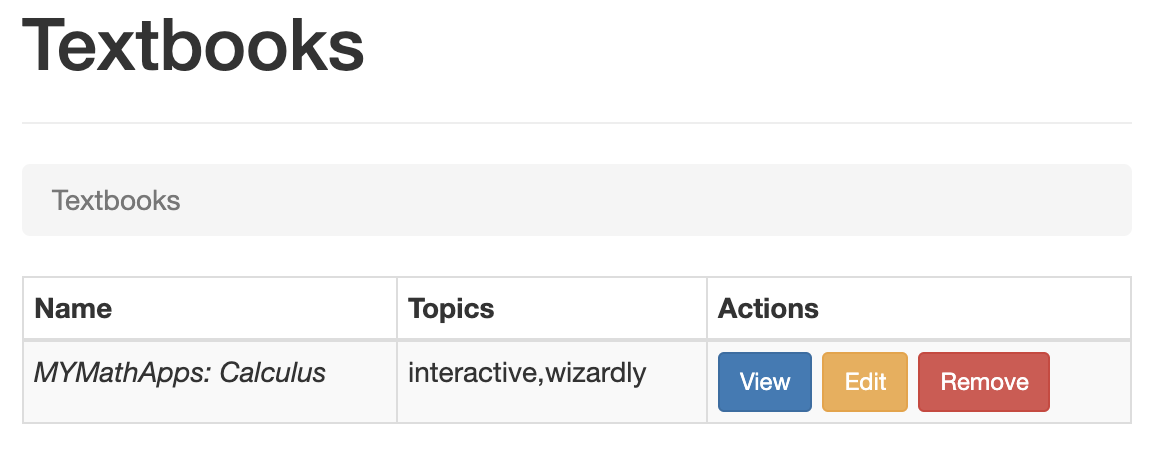
\includegraphics[scale=0.5]{textbooks.png}
    \caption[Textbook selection.]{The selection and upload of networks for a given textbook}
        
    \label{fig:textbooks}
\end{figure}

The next piece of the platform is the most important. It the actual piece of the platform that allows a consumer to reorder and restructure the original ordering of the textbook. It is fully interactive and draggable. Each unit and sub unit can be toggled to view more or less about units. There is also a button to toggle all units to be viewed or to collapse all units until only the independent root units are viewable.

\begin{figure}[ht]
    \centering
    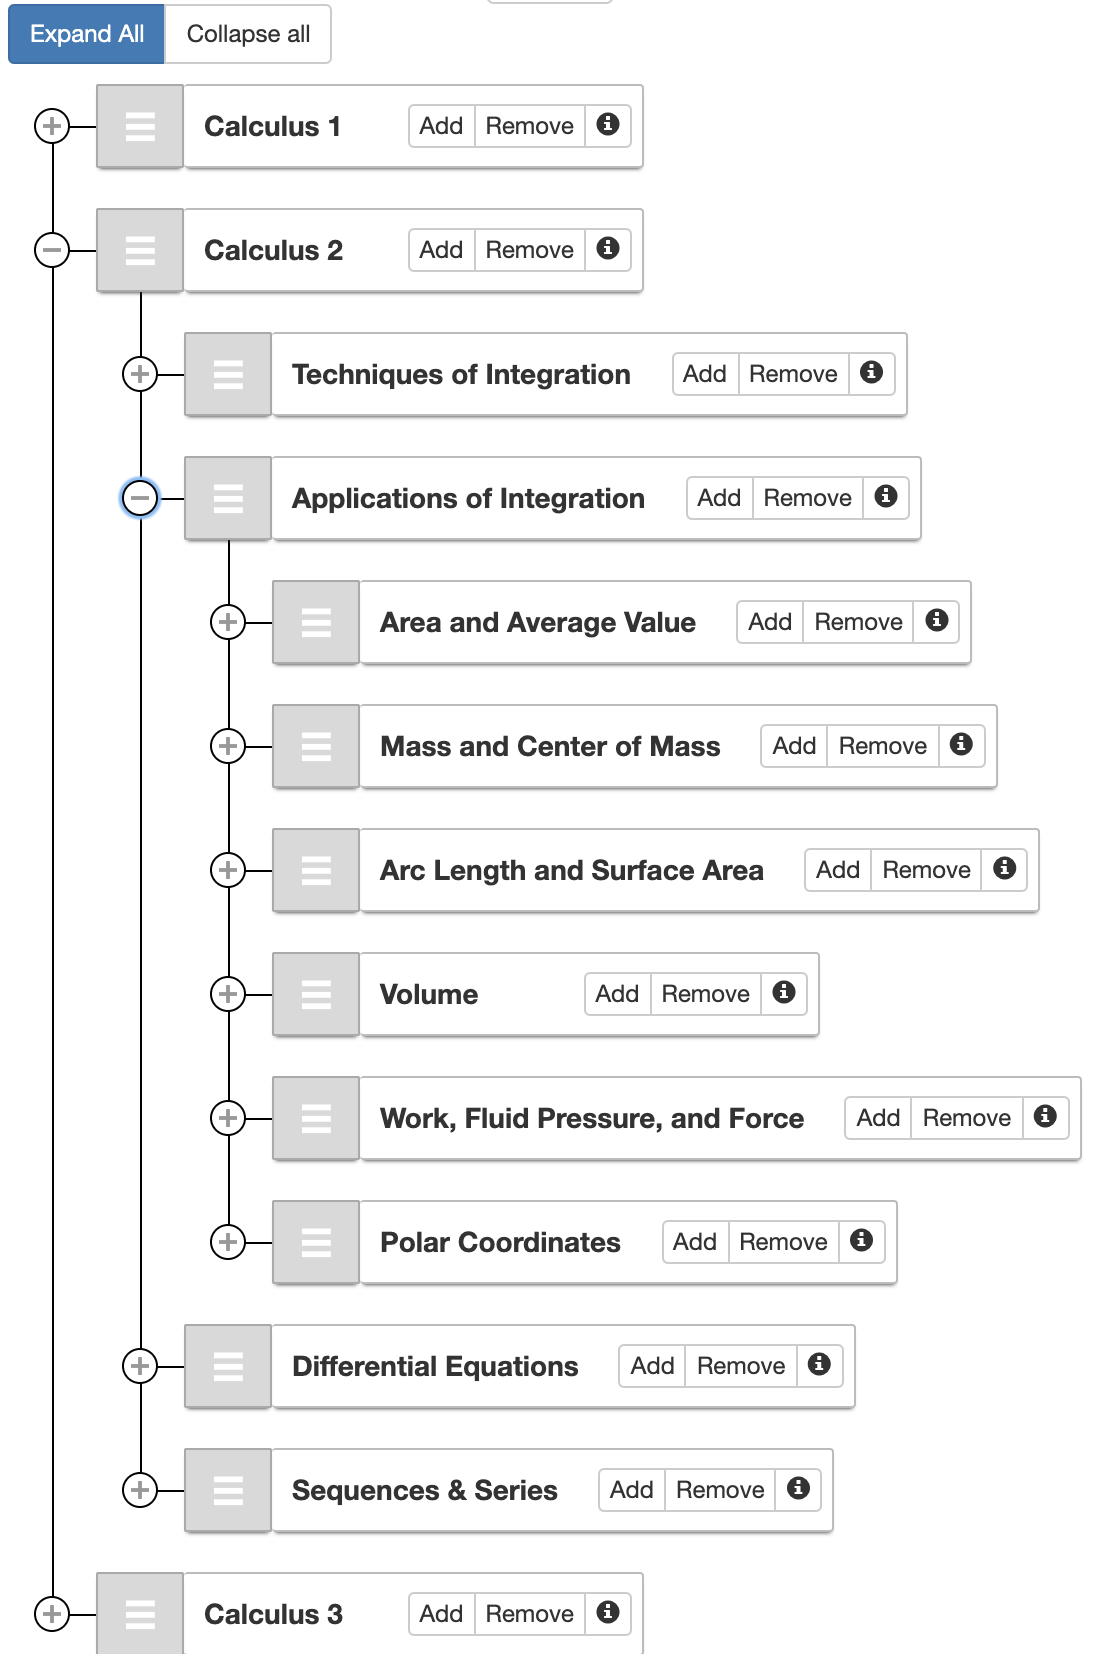
\includegraphics[scale=0.3]{nestedChapters.png}
    \caption[Unit hierarchy.]{Unit hierarchy.}
        
    \label{fig:nestedChapters}
\end{figure}

\pagebreak

On top of being toggleable, each unit is draggable Fig \ref{fig:chaptersMoving}. This allows for each unit to be moved to any other point in the structure of the tree or table of contents. During each of these movements, a request is sent to the server to check the and verify that all dependencies are met. If any dependency is not met, a message is then sent to the front end for it to be displayed to the user.

\begin{figure}[ht]
    \centering
    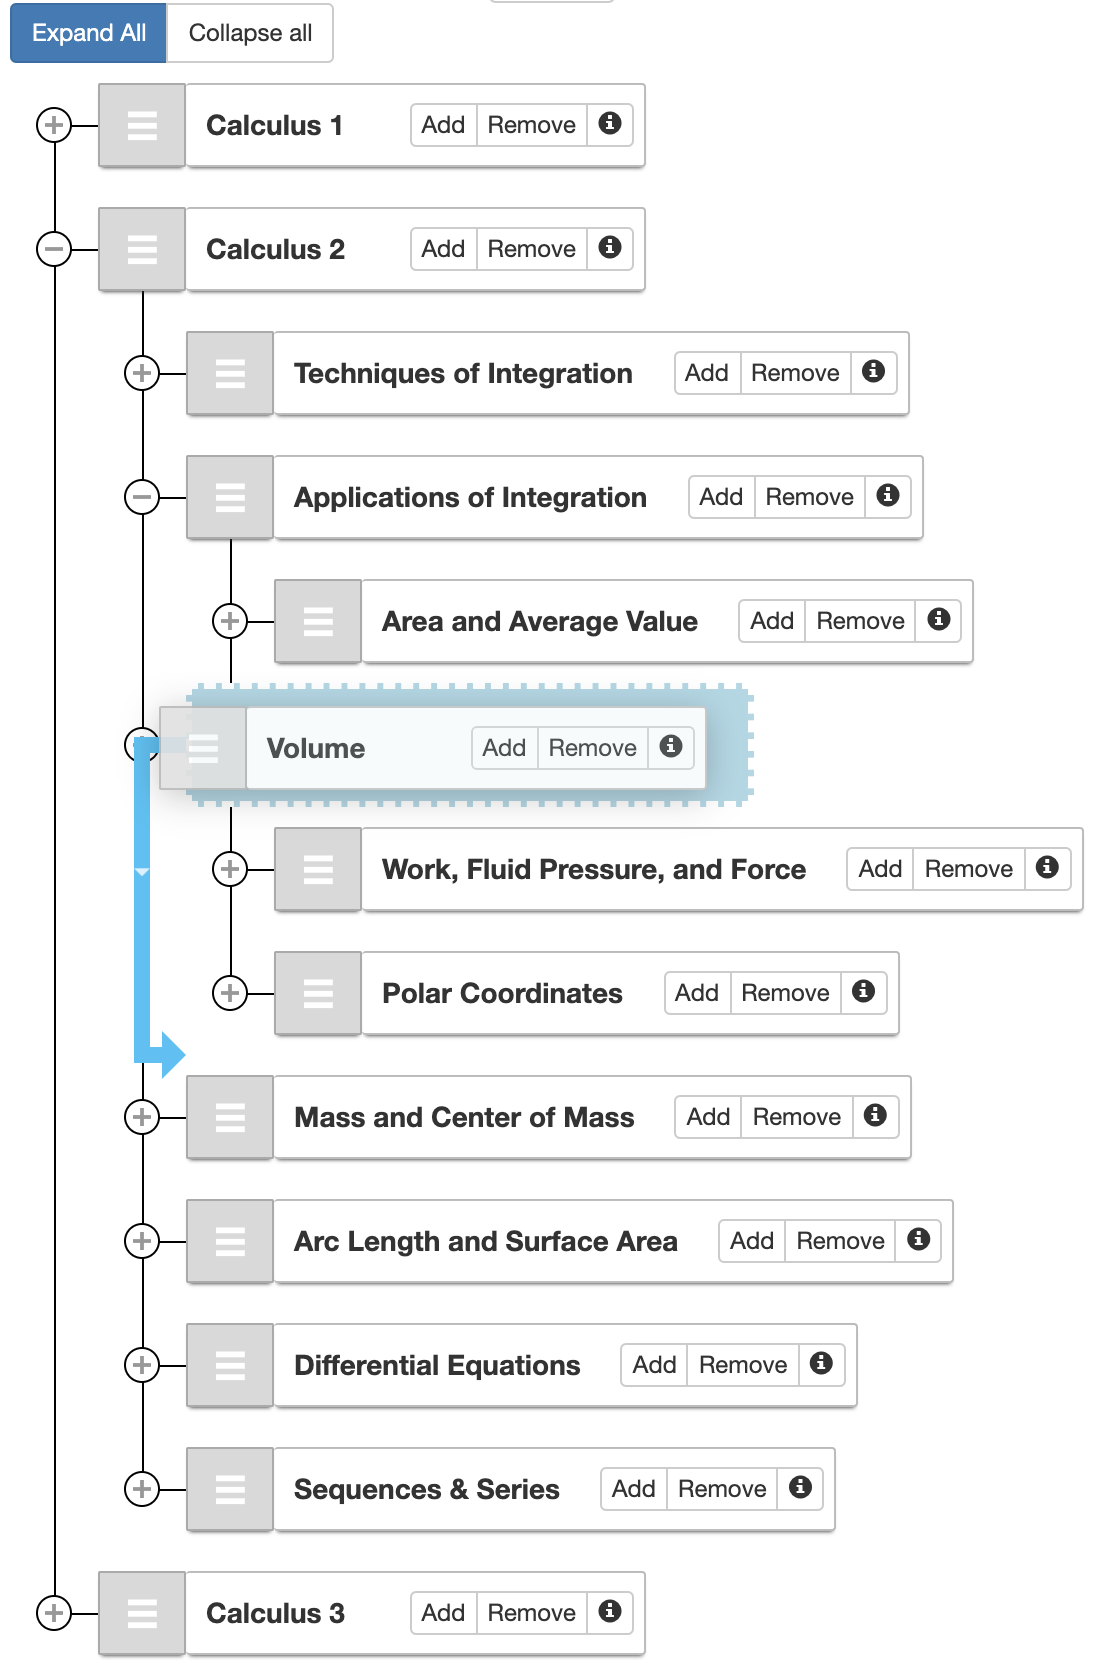
\includegraphics[scale=0.3]{chaptersMoving.png}
    \caption[Reordering units.]{Reordering of units through the use of dragging.}
        
    \label{fig:chaptersMoving}
\end{figure}

\pagebreak

%%%%%%%%%%%%%%%%%%%%%%%%%%%%%%%%%%%%%%%%%%%%%%%%%%%
%
%  New template code for TAMU Theses and Dissertations starting Fall 2016.
%
%
%  Original Author: Sean Zachary Roberson
%  This version adapted for URS by Parasol lab.
%  Adapted from version 3.16.10, which was last updated on 9/29/2016.
%  URS adaptation last updated 1/9/2017.
%
%%%%%%%%%%%%%%%%%%%%%%%%%%%%%%%%%%%%%%%%%%%%%%%%%%%
%%%%%%%%%%%%%%%%%%%%%%%%%%%%%%%%%%%%%%%%%%%%%%%%%%%%%%%%%%%%%%%%%%%%%%%
%%%                           ALGORITHM
%%%%%%%%%%%%%%%%%%%%%%%%%%%%%%%%%%%%%%%%%%%%%%%%%%%%%%%%%%%%%%%%%%%%%%

\chapter{THE ALGORITHM}


\section{Introduction}

The core portion of the platform that will allow reordering of aspects of the textbook can simply summed up as \textit{The Algorithm}. This underlying algorithm is independent of the technology or implementation. It is simply a high level description and analysis of the proposed solution to the given problem.

With an understanding of the algorithm, the implementation should follow in a natural and simple manner.

\section{Motivation for the Algorithm}

The algorithm has other items to consider outside simply just solving the given issue. As with most algorithms, there is a thought and focus on completing the desired task in an efficient and optimal manner. This means that if the algorithm is able to provide feedback but if it is done in an clunky manner, the algorithm is still considered a failure and not useful.

In addition to efficiency, correctness is another major point of focus. In this context, correctness relates to properly conveying the thoughts and concerns of the original author to the editor trying to modify the order of a textbook. As a result of a particular action or modification by the editor, there should never arise a situation where a suggestion or warning provided by the algorithm conflicts with the thoughts or viewpoints of the original author of the textbook. These messages provided by the algorithm should be simply an extension of the original if not exactly the same as if the author was at the computer sitting with the user of the platform.

Correctness also relates to truly reordering the textbook as desired and specified by the one who modified the order of the textbook. After a change by the editor, they should be able to clearly understand what type of change they are proposing, how this affects the textbook as a whole, how nearby sections or chapters may be affected and finally after committing these changes, the actual textbook should properly reflect these changes as desired by the editor. 

\section{The Design}

\subsection{Structure}

The design first has to answer the question of what. What information is necessary  to properly accomplish the given task. At the root of everything, there is the interdependency of topics. This is the core dependency upon which all other dependencies are built upon or derived from. All the following data types all directly or indirectly are tied to a particular topic or group of topics. A unit is very generic and could designate several different types. A unit is either a book, part, chapter, section, page or cul-de-sac. For the purpose of dependency mapping, there has not been a use case that distinctly separates the types of units for the purpose of dependency mapping. So they have been simply grouped together into type unit. An assessment is a tutorial or exercise providing a problem that is given to a student to solve. These are different from the units because of how they are presented and how the underlying content is used. A unit is simply a presentation of content and/or topics to the reader. An assessment is a formal way of allowing students to practice their skills and test the students knowledge. Another special consideration of assessments is their dynamic and flexible nature. Unit structure is what the editor will likely spend a majority of time reordering and tweaking. Once the unit structure is in place, the assessments should automatically reorder and populate to the correct units given the new unit dependency mapping. For the purpose of relating these two, a unique id is assigned to each topic, unit and assessment.

The next topic of focus is how to properly structure the necessary information to complete the given task. Since this is in fact a hierarchical dependency mapping problem at its core, a directed acyclic graph (DAG) was chosen to map and store the dependencies. The reason being because a given topic can have one of two true relations and one metarelation with any another topic. A given topic may depend on another topic because material must first be introduced in the latter topic in order to properly deliver the content in the former topic. This is an example of a child relationship. The reverse relation is also a relationship. This reverse relationship is an example of a parent relationship Fig \ref{fig:parent_child}.

\begin{figure}[ht]
    \centering
    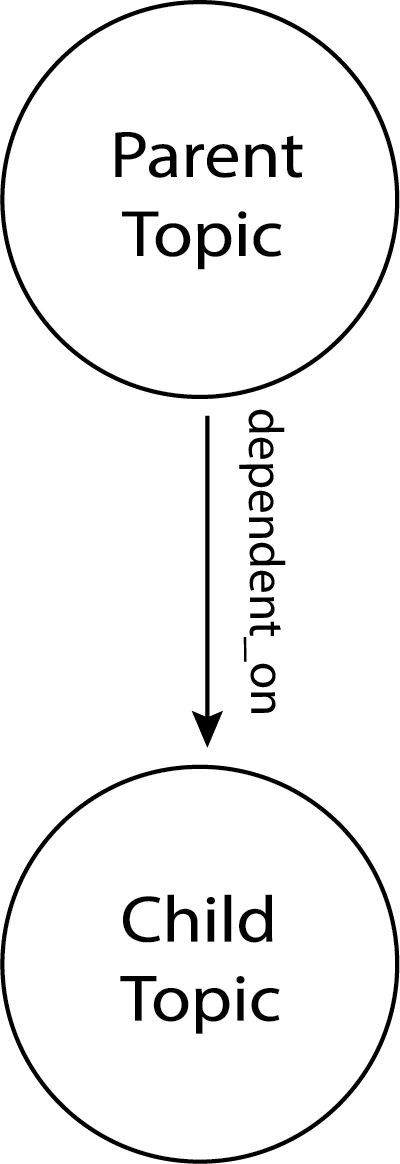
\includegraphics[scale=0.75]{parent_child.png}
    \caption[parent child topic.]{Parent child topics.}

    \label{fig:parent_child}
\end{figure}

Finally, the metarelation is the situation where two topics are located on similar levels of the hierarchy in the dependency mapping and do not have a parent or child relationship with one another. These topics are independent of one another, meaning that the order of these two topics in no way affect one another Fig \ref{fig:unrelated_topics}.

\pagebreak
\begin{figure}[ht]
    \centering
    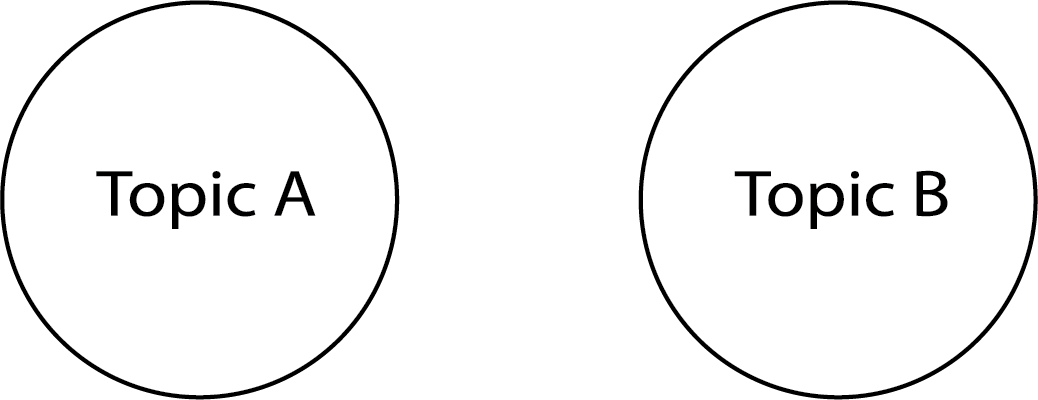
\includegraphics[scale=0.75]{unrelated_topics.png}
    \caption[Unrelated topics.]{Unrelated topics. Can have any number of parents and children but do not relate to one another.}
        
    \label{fig:unrelated_topics}
\end{figure}

The previous dependency mapping completely describes the requirements for mapping topics but units and assessments require more mappings.

Units have two relationships to map too. A particular unit can introduce one or more topics. However, units can also depend on other units. A given unit then depends on $N$ topics and $M$ units. A list of unique ids of these $N$ topics and $M$ units are stored on the unit node Fig \ref{fig:units}.

\begin{figure}[ht]
    \centering
    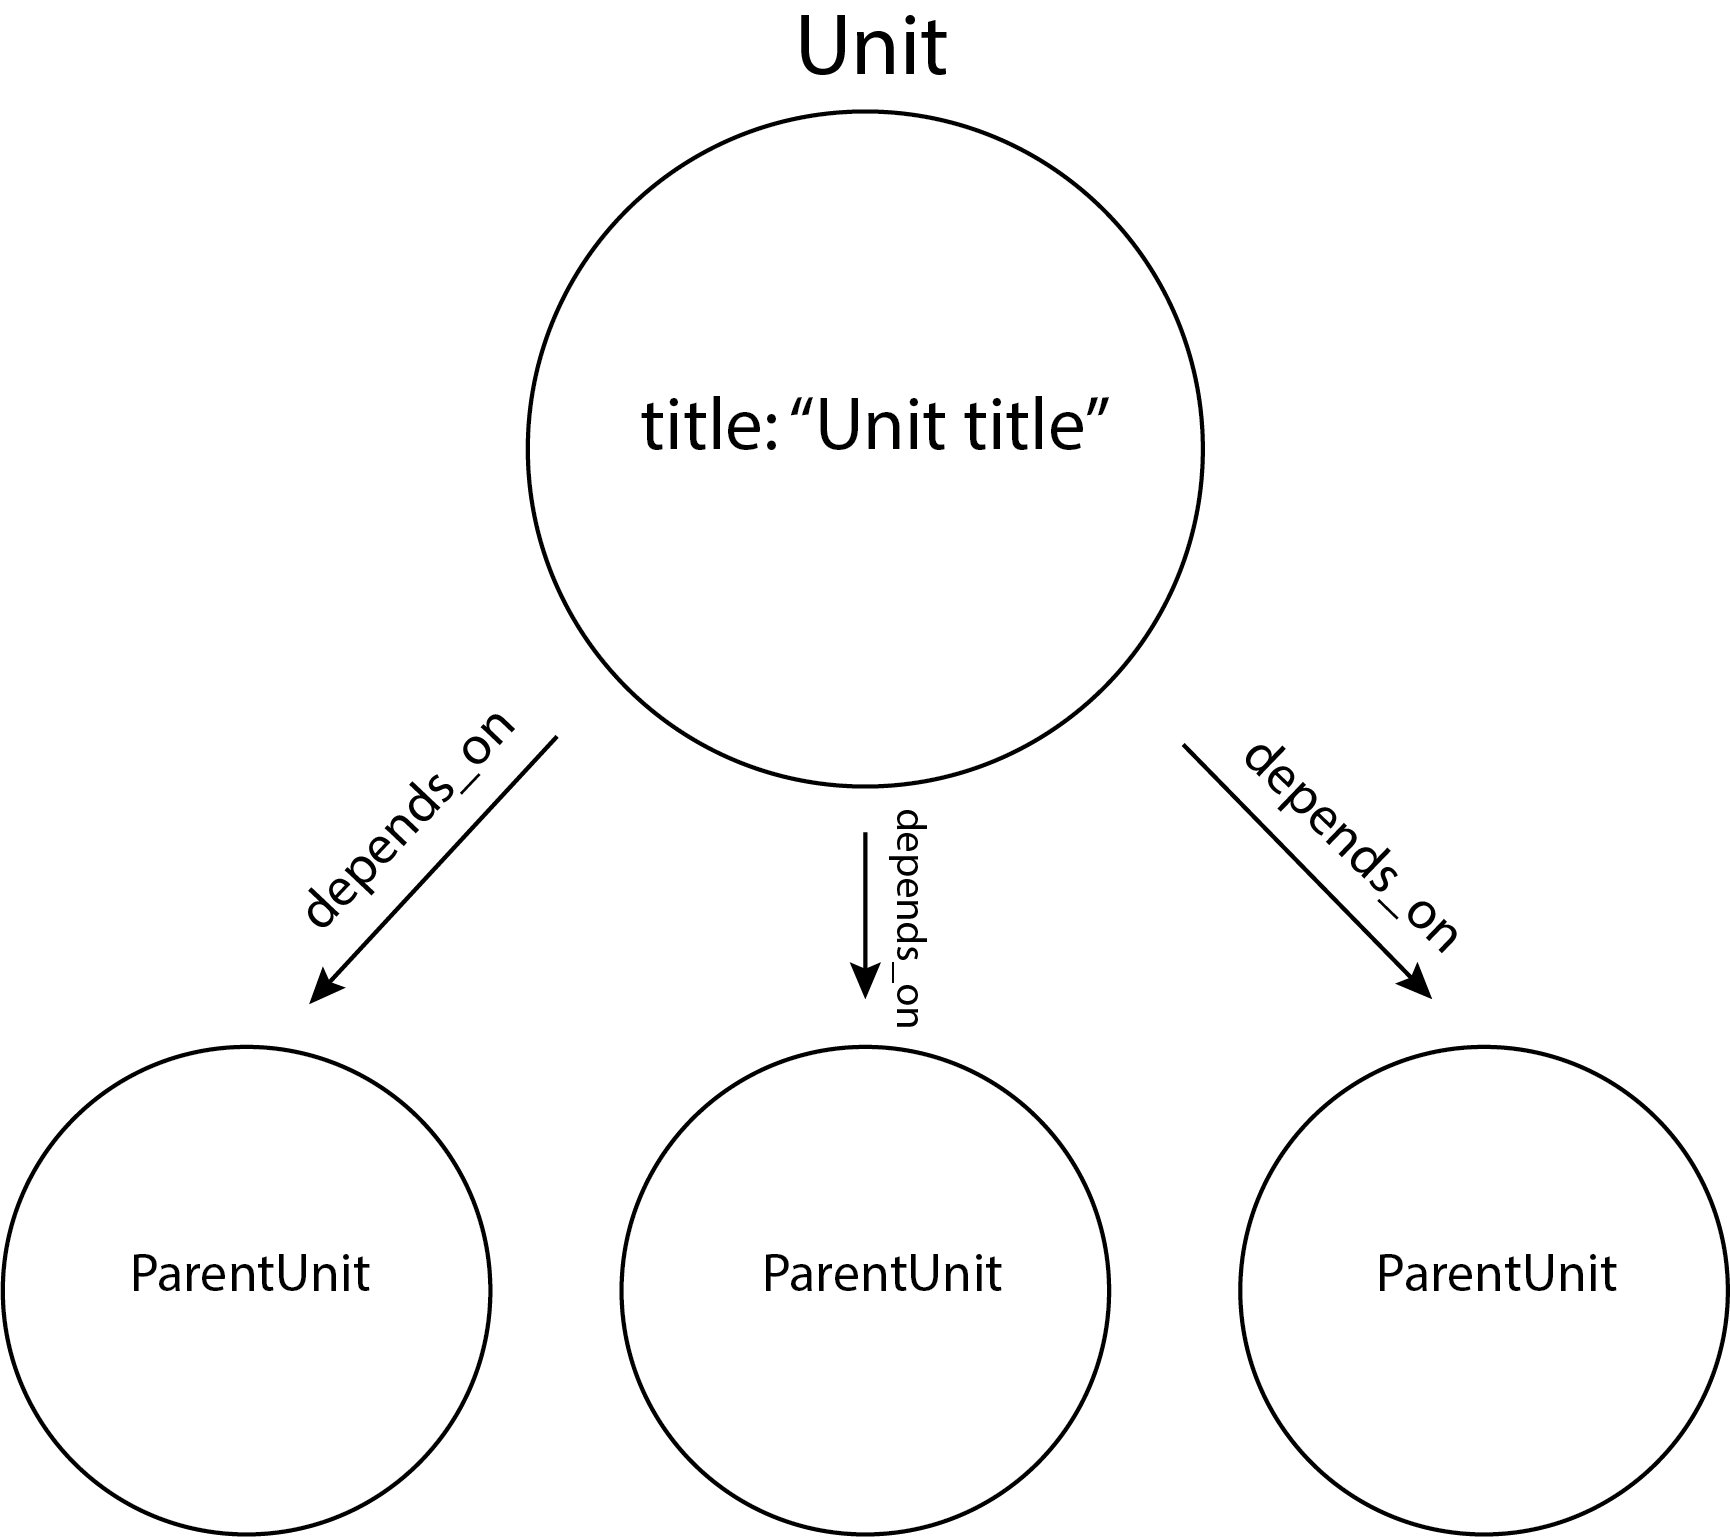
\includegraphics[scale=0.5]{units.png}
    \caption[Unit mapping.]{Unit mapping.}
        
    \label{fig:units}
\end{figure}

The final mapping is for the assessment data type. Assessments have three different possible data types it can depend on. They can depend on a topic, a unit or another assessment. The topic and unit dependency should ideally be the same but for our purposes, both must be satisfied in order for this dependency to be satisfied. In the absence of one, specifically the topic dependency, the other can be used. This is because if the topic dependency is missing for an assessment but unit dependencies are listed, the topic dependency can be generated by traversing the unit dependency mapping for the given units the assessment depends on. The final dependency on assessments is independent of topic or unit. The situation for assessment dependency arises when the results of one assessment is used in another assessment. In this situation, a given assessment should follow immediately after the dependent assessment or after another assessment that shares the same dependency on the same assessment.

Outside of dependency mapping, there is the actual order of the textbook and order of assessments. They can be contained with a DAG much like all the other mappings. These are what actually describes how the textbook will actually be ordered. These mappings are the only ones that are mutated for the sole purpose of reordering a textbook. There is a base mapping that is initially defined by the author for the first publication of the book. These base mappings should be structured in a way such that all dependencies are satisfied.

Finally it must be formally defined what \textit{satisfying all dependencies} means. In short, a unit or assessment satisfies it's dependencies when its position in the book occurs after all of its dependencies. The book satisfies all of its dependencies when all of its units and assessments satisfy their dependencies.

\subsection{Flow}

For a textbook that is going to be integrated into this dynamic modification flow, several dependency trees/DAGs need to be laid out describing the textbook. Specifically the different orderings as defined by the original author and an editor and how they interact with one another must be laid out. They are as follows.

\begin{enumerate}
    \item Net of topic interdependency (created by author)
    \item Net of unit interdependency $+$ topic dependency (created by author)
    \item Net of assessment interdependency $+$ topic or unit dependency (created by author)
    \item \begin{enumerate}
        \item Net of unit ordering (created by author)
        \item Net of unit ordering (created by editor)
    \end{enumerate}
    \item \begin{enumerate}
        \item Net of assessment ordering (created by author)
        \item Net of assessment ordering (created by editor)
    \end{enumerate}
\end{enumerate}

The workflow is as follows.

\begin{enumerate}
    \item Original author creates nets 1, 2 and 3 during or upon completion of writing the textbook. Nets 1, 2 and 3 should not be modified for the current version of the textbook. A modification of nets 1, 2 or 3 should be done to correct a dependency mistake or to add or rewrite a unit or topic. These modifications may result in a new edition of the textbook. These should be checked to see if all dependencies are satisfied.
    \item Nets 4a and 5a are automatically generated from nets 1, 2 and 3.
    \item The editor specifies the desired ordering of the revised textbook by modifying net 4a to produce net 4b.
        \begin{enumerate}
            \item During this process warnings are provided to the editor if any of their modifications in net 4b cause a dependency to not be met as defined in nets 1, 2 and 3.
        \end{enumerate}
    \item Using nets 1, 2 and 3 as well as the user modified net 4b, net 5b is generated defining the order of the assessments.
        \begin{enumerate}
            \item The editor can preview each assessment and modify the order in which it appears.
            \item During this process, warnings may be provided to the user if any of their modifications in net 5b cause a dependency to not be met as defined in nets 1, 2, 3 and 4b.
        \end{enumerate}
    \item The newly generated order in the form of nets 4b and 5b can then be utilized to modify the text and links in the given textbook.
\end{enumerate}

%%%%%%%%%%%%%%%%%%%%%%%%%%%%%%%%%%%%%%%%%%%%%%%%%%%
%
%  New template code for TAMU Theses and Dissertations starting Fall 2016.
%
%
%  Original Author: Sean Zachary Roberson
%  This version adapted for URS by Parasol lab.
%  Adapted from version 3.16.10, which was last updated on 9/29/2016.
%  URS adaptation last updated 1/9/2017.
%
%%%%%%%%%%%%%%%%%%%%%%%%%%%%%%%%%%%%%%%%%%%%%%%%%%%
%%%%%%%%%%%%%%%%%%%%%%%%%%%%%%%%%%%%%%%%%%%%%%%%%%%%%%%%%%%%%%%%%%%%%%
%%                           SECTION III
%%%%%%%%%%%%%%%%%%%%%%%%%%%%%%%%%%%%%%%%%%%%%%%%%%%%%%%%%%%%%%%%%%%%%



\chapter{THE IMPLEMENTATION}

% Notice that the title of this section is long - much longer than the others. When you have long section titles, this template takes care of double spacing the lines in the title. If the title is long to fit in the table of contents, the template will single space the title.

% \section{Yet Another Table}

% Another table is placed here to show the effect of having tables in multiple sections. The list of tables should still double space between table titles, while single spacing long table titles.

% %Fix table labeling.
% \begin{table}[h!]
% 	\centering
% 	\caption{San Japan attendance. Data is taken from \cite{ANCONS}. I intentionally make the title of this table long so the single space effect is seen in the list of tables.}
%         \vspace{1em}
% 	\begin{tabular}{|l|l|}
% 		\hline
% 		Dates & Attendance  \\ \hline
% 		August 8-10, 2008 & 3,523  \\ \hline
% 		August 14-16, 2009 & 4,003 \\ \hline
% 		July 9-11, 2010 & 5,049 \\ \hline
% 		August 5-7, 2011 & 6,891  \\ \hline
% 		August 10-12, 2012 & 9,464  \\ \hline
% 		August 16-18, 2013 & 11,077  \\ \hline
% 		July 18-20, 2014 & 14,686 \\ \hline
% 		July 31-August 2, 2015 & 18,411  \\ \hline
% 	\end{tabular}
% \end{table}

% You may be wondering why San Japan was chosen. There are a few reasons as to why I did this:

% \begin{enumerate}
% \item It is one of the fastest-growing anime conventions in Texas.
% \item Filler.
% \item I wanted a good variety of table examples.
% \item Because conventions are cool.
% \end{enumerate}

% The \textit{enumerate} environment was used to generated an ordered list above.

% \section{Section Test Example}
% We insert another figure here, just for kicks.

% \begin{figure}[h!]
% 	\centering
% 	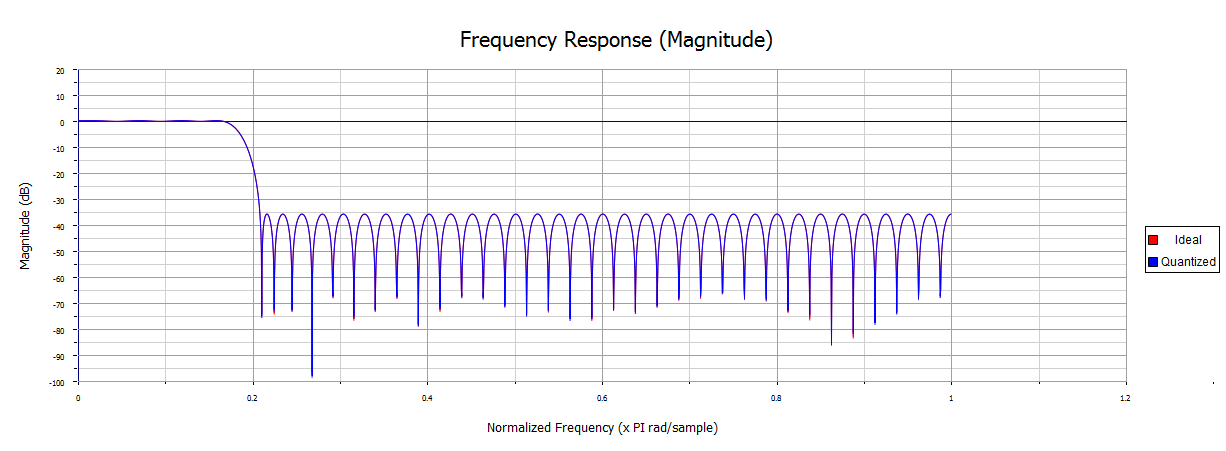
\includegraphics[scale=0.5]{LowPass_Filter_Design.png}
% 	\caption{A low pass filter design.}
% \end{figure}

%%%%%%%%%%%%%%%%%%%%%%%%%%%%%%%%%%%%%%%%%%%%%%%%%%%
%
%  New template code for TAMU Theses and Dissertations starting Fall 2016.
%
%
%  Original Author: Sean Zachary Roberson
%  This version adapted for URS by Parasol lab.
%  Adapted from version 3.16.10, which was last updated on 9/29/2016.
%  URS adaptation last updated 1/9/2017.
%
%%%%%%%%%%%%%%%%%%%%%%%%%%%%%%%%%%%%%%%%%%%%%%%%%%%
%%%%%%%%%%%%%%%%%%%%%%%%%%%%%%%%%%%%%%%%%%%%%%%%%%%%%%%%%%%%%%%%%%%%%%
%%                           SECTION IV
%%%%%%%%%%%%%%%%%%%%%%%%%%%%%%%%%%%%%%%%%%%%%%%%%%%%%%%%%%%%%%%%%%%%%

\chapter{CONCLUSION}

\section{Results}

Images of the application and textbook?

\section{Challenges}

Time? Tweaking existing build process of textbook for integration.

\section{Broader Impact}

Allow other authors to utilize this design + implementation?

\section{Future Plans}

Get this functional for entire MYMACalc book



%fix spacing in bibliography, if any...
%%%%%%%%%%%%%%%%%%%%%%%%%%%%%%%%%%%%%%%%%%%%%%%%%%%%%%%%%%%%%
%\let\oldbibitem\bibitem
%\renewcommand{\bibitem}{\setlength{\itemsep}{0pt}\oldbibitem}
%%%%%%%%%%%%%%%%%%%%%%%%%%%%%%%%%%%%%%%%%%%%%%%%%%%%%%%%%%%%%%%
%The bibliography style declared is the IEEE format. If
%you require a different style, see the document
%bibstyles.pdf included in this package. This file,
%hosted by the University of Vienna, shows several
%bibliography styles and examples of in-text citation
%and a references page.

\phantomsection
\addcontentsline{toc}{chapter}{REFERENCES}

\renewcommand{\bibname}{{\large\rm\bf REFERENCES}}
%This file is a .bib database that contains the sources.
\bibliographystyle{ieeetr}
\bibliography{data/myReference}

%This next line includes appendices. The file
%appendix.tex contains commands pointing to
%the appendix files; be sure to change these
%pointers if you end up changing the filenames.
%Leave this commented if you will not need
%appendix material.

% %%%%%%%%%%%%%%%%%%%%%%%%%%%%%%%%%%%%%%%%%%%%%%%%%%%
%
%  New template code for TAMU Theses and Dissertations starting Fall 2016.
%
%
%  Original Author: Sean Zachary Roberson
%  This version adapted for URS by Parasol lab.
%  Adapted from version 3.16.10, which was last updated on 9/29/2016.
%  URS adaptation last updated 1/9/2017.
%
%%%%%%%%%%%%%%%%%%%%%%%%%%%%%%%%%%%%%%%%%%%%%%%%%%%

% These are the commands to create an Appendix


%%%%%%%%%%%%%%%%%%%%%%%%%%%%%%%%%%%%%%%%%%%%%%%%%%%%%%%%%%%%%%%%%%%%%%
%%                           APPENDIX A
%%%%%%%%%%%%%%%%%%%%%%%%%%%%%%%%%%%%%%%%%%%%%%%%%%%%%%%%%%%%%%%%%%%%%

\phantomsection

\chapter*{First Appendix}
\addcontentsline{toc}{chapter}{\uppercase{First Appendix}}

Text for the Appendix follows.

\begin{figure}[h]
\centering
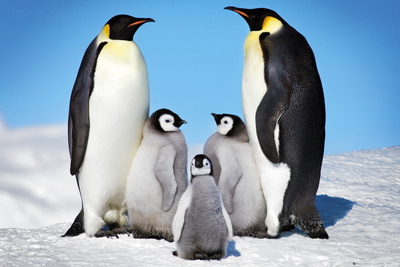
\includegraphics[scale=.50]{graphic/Penguins.jpg}
\caption{TAMU figure}
\label{fig:tamu-fig5}
\end{figure}

%%%%%%%%%%%%%%%%%%%%%%%%%%%%%%%%%%%%%%%%%%%%%%%%%%%%%%%%%%%%%%%%%%%%%%
%%                           APPENDIX B
%%%%%%%%%%%%%%%%%%%%%%%%%%%%%%%%%%%%%%%%%%%%%%%%%%%%%%%%%%%%%%%%%%%%%
\chapter*{A Second Appendix Whose Title Is Much Longer Than The First}
\addcontentsline{toc}{chapter}{\uppercase{A Second Appendix Whose Title Is Much
Longer Than The First}}

Text for the Appendix follows.

\begin{figure}[h]
\centering
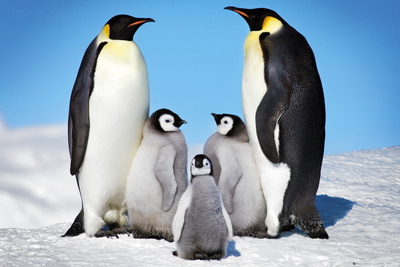
\includegraphics[scale=.50]{graphic/Penguins.jpg}
\caption{Another TAMU figure.}
\label{fig:tamu-fig6}
\end{figure}


\pagebreak{}

\end{document}
